%----------------------------------------------------------------------------------
% Exemplo do uso da classe tcc.cls. Veja o arquivo .cls
% para mais detalhes e instruções.
%----------------------------------------------------------------------------------
\chapter{\label{chap:chap2}Fundamentação Teórica}


\section{Prevenção de Colisão}
% Huang2020Ship.pdf
Uma tarefa primordial quando se trata de navegação é evitar que a embarcação colida com algum obstáculo. Porém, é alto o número de acidentes com embarcações envolvendo colisões. Além disso, diversas investigações apontam que a principal causa desses acidentes é o fator humano.

Frente ao alto número de ocorrencias dessa natureza, pesquisadores veem estudando meios de evitar tais acidentes. [Huang] afirma que atualmente há duas frentes na tecnologia de prevenção de colisão: (1) assitência à tripulação e (2) eliminação de fatores humanos. Sendo esta última a perspectiva abordada neste trabalho dado que o componente físico de implementação é um USV.

Huang (2020, p.2) define prevenção de colisão como:
\begin{directcite}
    \textit{"Prevenção de colisão é o processo em que um navio desvia de sua trajetória planejada para evitar contato físico indesejado em um certo tempo futuro"}
\end{directcite}

Com isso, [Huang] separa o processo de prevenção de colisão nas etapas de "detecção de conflito", que determina se o navio está em risco de colisão ou não, e "resolução de conflito", que define quais ações devem ser tomadas pelo navio para evitar a colisão. Em um USV, tais atividades são atribuidas ao módulo de \textit{"Guidance"} do sistema GNC.

%EXPLICAR SISTEMA GNC NO CAPÍTULO DE USV

Em um USV tais atividades são atribuidas ao sistema GNC (do inglês \textit{"Guidance Navigation and Control"}), mais especificamente ao módulo de \textit{"Guidance"}. Os módulos de \textit{"Navigation"} e \textit{"Control"} são responsáveis por fornecer informações a respeito do arredor do navio ao módulo de \textit{"Guidance"} e executar as ações definidas pelo módulo de \textit{"Guidance"}, respectivamente.

De acordo com a ~\ref{fig:decision_process}

\begin{figure}
    \centering
    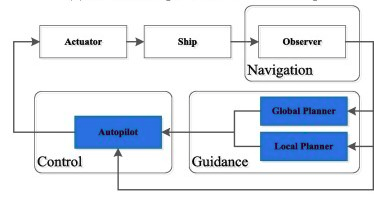
\includegraphics{fig/decision_process.png}
    \caption{Processo de decisão em um USV ~\cite{HUANG2020451}}
    \label{fig:decision_process}
\end{figure}

\subsection{}